%
% File naaclhlt2013.tex
%

\documentclass[11pt,letterpaper]{article}
\usepackage{naaclhlt2013}
\usepackage{times}
\usepackage{multirow}
\usepackage{latexsym}
\usepackage{graphicx}
\graphicspath{{images/}}
\setlength\titlebox{6.5cm}    % Expanding the titlebox

\title{TEA: Temporal Entity Annotator}

%\Thanks{This
%    document has been adapted from the instructions for earlier ACL
%    and NAACL proceedings, including those for
%    NAACL-HLT-12 by Nizar Habash and William Schuler,
%    NAACL-HLT-10 by Claudia Leacock and Richard Wicentowski,
%    NAACL-HLT-09 by Joakim Nivre and Noah Smith,
%    for ACL-05 by Hwee Tou Ng and Kemal Oflazer,
%    for ACL-02 by Eugene Charniak and Dekang Lin, and earlier ACL and
%    EACL formats.  Those versions were written by several people,
%    including John Chen, Henry S. Thompson and Donald Walker.
%    Additional elements were taken from the formatting instructions of
%    the {\em International Joint Conference on Artificial Intelligence}.
%    This second version clarifies the procedure for
%    submitting for double-blind reviewing.}}

\author{Kevin Wacome\\
	    University of Massachusetts Lowell\\
	    1 University Ave\\
	    Lowell, MA 01854, USA\\
	    Kevin\_Wacome@student.uml.edu\\
	  \And
		Connor Cooper\\
	  	University of Massachusetts Lowell\\
	  	1 University Ave\\
	  	Lowell, MA 01854, USA\\
		Connor\_Cooper@student.uml.edu\\}

\date{2 Oct 15}

\begin{document}
\maketitle
\begin{abstract}
Temporal Entity Annotator (TEA) is a reimplementation of the system described by the SemEval-2015 Task-5 challenge winners. This tasks involves extracting temporal relation, temporal expressions, and event entities for the purpose of Question Answering. To achieve this, TEA is composed of a series of Support Vector Machine (SVM) classifiers, with one classifier for each extraction component. TEA obtained a recall score of <INSERT RECALL SCORE HERE ONCE WE HAVE ONE> over the entire test data set, opposed to the 0.30 achieved by task winner's system.
\end{abstract}

\section{Problem Overview}

The goal of this project is to implement a baseline system that performs as well as the best competitors for the SemEval 2015 challenge titled QA TempEval. This will provide a starting point for research into ways to improve performance of temporal relation extraction. The system is required to annotate tokens within TE3Input files, which are a special class of TimeML file that lacks full temporal annotation, but contains certain annotations such as document creation time. These tokens are annotated as either TIMEX3 temporal expressions or events. Temporal relations are then identified between event/event and event/TIMEX3 pairs.\cite{Llorens:15}.


\section{Relevant Literature and Related Works}

TimeML is a markup specification that is used to represent temporal entities with the aims of providing a rich and informative representation to allow for accurate automatic recognition of temporal relations between entities by software systems \cite{Pustejovsky:03}. According to the TimeML specification, temporal entities are broken down into temporal expressions and events. Events are described as occurrences of situations and states and temporal expressions represent moments in time or durations. Temporal relations are described as the link between related entities that places them in a relative time frame to one another, such as preceding or occurring after.

Part of the challenge of this SemEval task is to create meaningful annotations that allow the QA system provided by the organizers to answer questions accurately. In the proceedings from SemEval 2015 \cite{Llorens:16}, a list of the systems that perform the best annotations was provided, some abstracts were also written describing the methods used to participate in this challenge. HLT-FBK was the system with the best general performance because it achieved on average the highest F-measure of all of the systems.

Two systems were ranked in the SemEval task out system is solving \cite{Llorens:16}. The HLT-FBK system, which our system is based on, ranked first, using a similar SVM based classification pipeline. The second place system, HITSZ-ICRC, utilized several other temporal annotation systems, and then fed them into a correction system. This correction system merged the output of the initial annotators. This system resulted in an F-measure of 0.12 over the test corpus, opposed to the 0.37 F-measure from the HLT-FBK system \cite{Llorens:16}. Both systems were evaluated with the QA system distributed for the QA TempEval SemEval task. While neither system received a particularly high F-measure for the task, the HLT-FBK system clearly outperforms the HITSZ-ICRC system. For this reason, this version of TEA has been designed as a reimplementation of the HLT-FBK system. 


\section{Data and Tools}

TEA is tested, trained, and evaluated using the data distributed for the QA TempEval Task. A QA kit is also distributed for testing our annotations. Training data is composed of 25 documents with TE3Input files, as well as TBAQ cleaned files from the TimeBank and AQUAINT corpora. These provide an additional 256 documents to train over. The test data contains 8 blog entries, 10 news articles, and 10 Wikipedia articles.

Several external tools were leveraged to obtain feature and process data for the system. \textbf{NewsReader} is used for the majority of preprocessing. The tokenization, part of speech (PoS) tagging, named entity recognition, constituency tree, and semantic role labeling modules were utilized. \textbf{CorefGraph} is used to preform coreference resolution. \textbf{AddDiscoure} is used to extract temporal discourse connectives for several features \cite{Pitler:09}. \textbf{Scikit-learn} is used to implement our classifiers. \textbf{TImeNorm} is used to obtain the value attribute of TIMEX3 entities when writing them to the output file.


\section{System Overview}

\noindent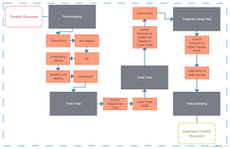
\includegraphics{rsz_tea}

\subsection{Preprocessing}

TEA's preprocessing pipeline is implemented using NewsReader and CorefGraph. From NewsReader, the IXA pipes modules are utilized to perform tokenization, part of speech tagging, named entity recognition, build constituency trees, and extract semantic role labels. The final portion of the pipeline is coreference resolution, extracted using CorefGraph. This outputs an NAF format xml document, which is then parsed to obtain relevant information for each token. This information is then stored to be passed to the classifiers later.

\subsection{Temporal Expression Extraction}

The extraction and classification of temporal expressions (timex) is solved as a text chunking task. Timex expressions are classified as either DATE, TIME, or DURATION. Timexes can span multiple tokens, so IOB labellings are used, resulting in the following seven classes from the classifier: B\_DATE, I\_DATE, B\_TIME, I\_TIME, B\_DURATION, I\_DURATION, and O, for tokens that are not part of a timex. Timexes are classified using a single Suport Vector Machine (SVM) classifier with a polynomial kernal.

All tokens are considered as candidates for timexes. Timexes are identified using the token's text, part of speech, whether the token is a member of a named entity, the four tokens to the left and right of the token in question, and whether the token matches a regular expression pattern for time units, part of a day, the name of a day, the name of a month, or a duration pattern. Once identified, timexes are normalized with TimeNorm, in accordance with the HLT-FBK system \cite{Mirza:15}.

\subsection{Event Extraction}

Event extraction is also taken as a text chunking task. Unlike the HLT-FBK system, which uses two classifiers to first identify events as either EVENT or O and then classify the events, TEA uses only one classifier to perform both tasks at once \cite{Mirza:15}. Events are classified as REPORTING, PERCEPTION, ASPECTUAL, ACTION, STATE, or OCCURRENCE. IOB labels are used to account for events which span multiple tokens, resulting in the following final labeling for the SVM classifier: B\_REPORTING, B\_PERCEPTION, B\_ASPECTUAL, B\_ACTION, B\_STATE, B\_OCCURRENCE, I\_REPORTING, I\_PERCEPTION, I\_ASPECTUAL, I\_ACTION, I\_STATE, I\_OCCURRENCE, or O for tokens that are not classified as events.

Every token that is not identified as a temporal entity is considered as a candidates for event classification. Events are identified using the token's text, part of speech, whether the token is part of a named entity, whether the token is the main verb of a sentence, whether the token is part of a temporal discourse connective, and the four tokens to the left and right of the token in question. Discourse connective information is obtained from the addDiscourse tool.

\subsection{Temporal Relation Extraction}

Temporal relation extraction is treated as a simple classification task across pairs of entities. The temporal links (TLINKs) are assigned one of 13 labels in accordance with the TimeML specification. However, in order to account for sparsity in the training data, only a subset of the original labels are used. Unused labels are mapped to other labels when encountered in training data, using the mappings shown below:

\vspace{5mm}

\begin{center}
	\begin{tabular}{ |c|c|c|c| } 
		\hline
		\textbf{Original TimeML Label} & \textbf{TEA Labeling Subset} \\
		\hline
		IDENTITY &  \\ 
		DURING & SIMULTANEOUS \\ 
		SIMULTANEOUS &  \\ 
		\hline
		IBEFORE & BEFORE \\
		BEFORE & \\
		\hline
		IAFTER & AFTER \\
		AFTER & \\
		\hline
		INCLUDES & IS\_INCLUDED \\
		IS\_INCLUDED & \\
		\hline
		BEGINS & BEGUN\_BY \\
		BEGUN\_BY & \\
		\hline
		ENDS & ENDED\_BY \\
		ENDED\_BY & \\
		\hline
		
	\end{tabular}
\end{center}

\vspace{5mm}

TLINKs are identified across TIMEX3/EVENT and EVENT/EVENT pairs. Only entities in the same sentence are considered as candidates for temporal relations, with a few notable exceptions. The document creation time (which servers as an anchor for all temporal expressions) is considered for relations with every event. Events containing the root verb of a sentence are also considered for pairing with events in the following sentence.

TLINKs are extracted using the following features: the labelings of each entity obtained from the previous two passes, whether the PoS tags of the entities are the same, how many sentences are between the entities (this is zero for most pairs, since most pairs considered are in the same sentence), how many entities occur between the two entities in the pair, whether an entity in the pairing is the document creation time, the tokens of any temporal discourse connectives that are between the entities, and the number of tokens between each entity and the temporal discourse connective (if one is present). The addDiscourse tool is used again to obtain temporal discourse connectives. Once all TLinks have been extracted, the annotations are written to a TimeML file in the systems output directory.


\section{Evaluation}

In accordance with the task description \cite{Llorens:15}, we will be using news, blog, and Wikipedia articles to test our system. The corpus will be tagged and then tested by the question answering system distributed with the test data. The task winner reached a recall score of .30 across all domains, with F1 scores between .25 and .46, depending on the domain \cite{Mirza:15}. 

OUR RESULTS GO HERE ONCE WE GET THEM.


\section{Results}

TEXT ABOUT RESULTS
\\TEXT is here to force tables to the next page, so that they appear in the left column.
\\TEXT\\TEXT
\\TEXT\\TEXT\\TEXT\\TEXT\\TEXT\\TEXT


\begin{center}
\begin{tabular}{c|cccc|cccc|cccc||c}

\multirow{2}{*}{} &
	\multicolumn{4}{c}{News} & 
	\multicolumn{4}{|c}{Wikipedia} & 
	\multicolumn{4}{|c||}{Blogs} & 
	\multicolumn{1}{c}{All Domains} \\
	
	& Cov & P & R & F1 
	& Cov & P & R & F1 
	& Cov & P & R & F1 
	& R\\
	\hline

	TEA & 
	0.00 & 0.00 & 0.00 & 0.00 & 
	0.00 & 0.00 & 0.00 & 0.00 & 
	0.00 & 0.00 & 0.00 & 0.00 & 
	0.00 \\

	HLT-FBK 1 &
	0.29 & 0.59 & 0.17 & 0.27 &
	0.29 & 0.55 & 0.16 & 0.25 &
	0.32 & 0.57 & 0.18 & 0.28 &
	0.17 \\
	
	HLT-FBK 2 &
	0.55 & 0.43 & 0.23 & 0.30 &
	0.50 & 0.52 & 0.26 & 0.35 &
	0.43 & 0.43 & 0.18 & 0.26 &
	0.23 \\
	
	HLT-FBK 3 &
	0.36 & 0.56 & 0.20 & 0.30 &
	0.29 & 0.58 & 0.17 & 0.26 &
	0.29 & 0.47 & 0.14 & 0.21 &
	0.17 \\
	
	HLT-FBK 4 &
	0.69 & 0.43 & 0.29 & 0.35 &
	0.58 & 0.62 & 0.36 & 0.46 &
	0.58 & 0.34 & 0.20 & 0.25 & 
	0.30 \\

\end{tabular}
\end{center}


\begin{center}
	\begin{tabular}{c|ccc|cc|ccc|cc|ccc|cc}
		
	\multirow{2}{*}{} &
		\multicolumn{5}{c}{News} & 
		\multicolumn{5}{|c}{Wikipedia} & 
		\multicolumn{5}{|c}{Blogs} \\
	
	\multirow{2}{*}{} &
		\multicolumn{3}{r}{Answered} &
		\multicolumn{2}{l|}{Unknown} &
		\multicolumn{3}{r}{Answered} &
		\multicolumn{2}{l|}{Unknown} &
		\multicolumn{3}{r}{Answered} &
		\multicolumn{2}{l}{Unknown} \\
		
		& Q & Cor & Inc & Ent & Rel
		& Q & Cor & Inc & Ent & Rel
		& Q & Cor & Inc & Ent & Rel \\
		\hline
	
		TEA & 
		0.00 & 0.00 & 0.00 & 0.00 & 0.00 &
		0.00 & 0.00 & 0.00 & 0.00 & 0.00 & 
		0.00 & 0.00 & 0.00 & 0.00 & 0.00 \\

		HLT-FBK 3 &
		99 & 20 & 16 & 17 & 46 &
		130 & 22 & 16 & 48 & 44 &
		65 & 9 & 10 & 22 & 24 \\

		HLT-FBK 4 &
		99 & 29 & 39 & 16 & 15 &
		130 & 47 & 29 & 48 & 6 &
		65 & 13 & 25 & 22 & 5 \\
		
	\end{tabular}
\end{center}

\vspace{5mm}

OUR DETAILED RESULTS AND EXPERIMENT OUTLINES GO HERE ONCE WE GET THEM


\section{Potential Improvements}

Aside from simply increasing the feature set to better represent the entities being extracted, there are several ways to improve the performance of a classification system. One such way, which has significant potential for this system, is joint inference. By creating a bi-directional information flow between each of the classifiers, we can reduce the errors that would normally accumulate through the pipeline. This will likely have significant benefit to the TIMEX3 and EVENT classifiers, which will in turn improve the quality of the TLINK classifier. This will allow us to make the most of the features we already have, rather than creating larger, more complex feature spaces.



%\section{Introduction}
%
%The following instructions are directed to authors of papers accepted
%for publication in the NAACL HLT 2013 proceedings.  All authors are required
%to adhere to these specifications. Authors are required to provide
%a Portable Document Format (PDF) version of
%their papers.  The proceedings will be printed on US-Letter paper.
%Authors from countries in which access to word-processing systems is
%limited should contact the publication chairs as soon as possible.

%\paragraph{What's new} This year, grayscale readability will be enforced for all accepted
%papers (\S\ref{ssec:accessibility}).  Apart from this, the style files and camera-ready requirements
%are unchanged from last year.

%\section{General Instructions}

%Manuscripts must be in two-column format.  Exceptions to the
%two-column format include the title, as well as the
%authors' names and complete
%addresses (only in the final version, not in the version submitted for review),
%which must be centered at the top of the first page (see
%the guidelines in Subsection~\ref{ssec:first}), and any full-width
%figures or tables.  Type single-spaced.  Do not number the pages.
%Start all pages directly under the top margin.  See the guidelines
%later regarding formatting the first page.

%% If the paper is produced by a printer, make sure that the quality
%% of the output is dark enough to photocopy well.  It may be necessary
%% to have your laser printer adjusted for this purpose.  Papers that are too
%% faint to reproduce well may not be included.

%% {\bf Do not print page numbers on the manuscript.}  Write them lightly
%% on the back of each page in the upper left corner along with the
%% (first) author's name.

%The maximum length of a manuscript is eight (8) pages for the main
%conference, printed single-sided, plus two (2) pages for references
%(see Section~\ref{sec:length} for additional information on the
%maximum number of pages).  Do not number the pages.

%The review process is double-blind, so do not include any author information (names, addresses) when submitting a paper for review.  However, you should allocate space for the names and addresses so that they will fit in the final (accepted) version.  This is best done by either providing fake or blank names and addresses (as shown in this paper).

%\subsection{Electronically-available resources}

%NAACL HLT provides this description in \LaTeX2e{} ({\tt naaclhlt2013.tex}) and PDF
%format ({\tt naaclhlt2013.pdf}), along with the \LaTeX2e{} style file used to
%format it ({\tt naaclhlt2013.sty}) and an ACL bibliography style ({\tt naaclhlt2013.bst}).
%These files are all available at
%{\tt http://naacl2013.naacl.org}.  A Microsoft Word
%template file ({\tt naaclhlt2013.dot}) is also available at the same URL. We
%strongly recommend the use of these style files, which have been
%appropriately tailored for the NAACL HLT 2013 proceedings.


%\subsection{Format of Electronic Manuscript}
%\label{sect:pdf}

%For the production of the electronic manuscript you must use Adobe's
%Portable Document Format (PDF). This format can be generated from
%postscript files: on Unix systems, you can use {\tt ps2pdf} for this
%purpose; under Microsoft Windows, you can use Adobe's Distiller, or
%if you have cygwin installed, you can use {\tt dvipdf} or
%{\tt ps2pdf}.  Note
%that some word processing programs generate PDF which may not include
%all the necessary fonts (esp. tree diagrams, symbols). When you print
%or create the PDF file, there is usually an option in your printer
%setup to include none, all or just non-standard fonts.  Please make
%sure that you select the option of including ALL the fonts.  {\em
%  Before sending it, test your {\/\em PDF} by printing it from a
%  computer different from the one where it was created}. Moreover,
%some word processor may generate very large postscript/PDF files,
%where each page is rendered as an image. Such images may reproduce
%poorly.  In this case, try alternative ways to obtain the postscript
%and/or PDF.  One way on some systems is to install a driver for a
%postscript printer, send your document to the printer specifying
%``Output to a file'', then convert the file to PDF.

%For reasons of uniformity, Adobe's {\bf Times Roman} font should be
%used. In \LaTeX2e{} this is accomplished by putting

%\begin{quote}
%\begin{verbatim}
%\usepackage{times}
%\usepackage{latexsym}
%\end{verbatim}
%\end{quote}
%in the preamble.

%Additionally, it is of utmost importance to specify the {\bf
%  US-Letter format} (8.5in $\times$ 11in) when formatting the paper.
%When working with {\tt dvips}, for instance, one should specify {\tt
%  -t letter}.

%Print-outs of the PDF file on US-Letter paper should be identical to the
%hardcopy version.  If you cannot meet the above requirements about the
%production of your electronic submission, please contact the
%publication chairs above  as soon as possible.


%\subsection{Layout}
%\label{ssec:layout}

%Format manuscripts two columns to a page, in the manner these
%instructions are formatted. The exact dimensions for a page on US-letter
%paper are:

%\begin{itemize}
%\item Left and right margins: 1 inch
%\item Top margin: 1 inch
%\item Bottom margin: 1 inch
%\item Column width: 3.15 inches
%\item Column height: 9 inches
%\item Gap between columns: 0.2 inches
%\end{itemize}

%\noindent Papers should not be submitted on any other paper size. Exceptionally,
%authors for whom it is \emph{impossible} to format on US-Letter paper,
%may format for \emph{A4} paper. In this case, they should keep the \emph{top}
%and \emph{left} margins as given above, use the same column width,
%height and gap, and modify the bottom and right margins as necessary.
%Note that the text will no longer be centered.

%\subsection{The First Page}
%\label{ssec:first}

%Center the title, author's name(s) and affiliation(s) across both
%columns (or, in the case of initial submission, space for the names).
%Do not use footnotes for affiliations.  Do not include the
%paper ID number assigned during the submission process.
%Use the two-column format only when you begin the abstract.

%{\bf Title}: Place the title centered at the top of the first page, in
%a 15 point bold font.  (For a complete guide to font sizes and styles, see Table~\ref{font-table}.)
%Long title should be typed on two lines without
%a blank line intervening. Approximately, put the title at 1in from the
%top of the page, followed by a blank line, then the author's names(s),
%and the affiliation on the following line.  Do not use only initials
%for given names (middle initials are allowed). Do not format surnames
%in all capitals (e.g., ``Bangalore,'' not ``BANGALORE'').  The affiliation should
%contain the author's complete address, and if possible an electronic
%mail address. Leave about 0.75in between the affiliation and the body
%of the first page.

%{\bf Abstract}: Type the abstract at the beginning of the first
%column.  The width of the abstract text should be smaller than the
%width of the columns for the text in the body of the paper by about
%0.25in on each side.  Center the word {\bf Abstract} in a 12 point
%bold font above the body of the abstract. The abstract should be a
%concise summary of the general thesis and conclusions of the paper.
%It should be no longer than 200 words.  The abstract text should be in 10 point font.

%{\bf Text}: Begin typing the main body of the text immediately after
%the abstract, observing the two-column format as shown in
%the present document.  Do not include page numbers.

%{\bf Indent} when starting a new paragraph. For reasons of uniformity,
%use Adobe's {\bf Times Roman} fonts, with 11 points for text and
%subsection headings, 12 points for section headings and 15 points for
%the title.  If Times Roman is unavailable, use {\bf Computer Modern
%  Roman} (\LaTeX2e{}'s default; see section \ref{sect:pdf} above).
%Note that the latter is about 10\% less dense than Adobe's Times Roman
%font.

%\subsection{Sections}

%{\bf Headings}: Type and label section and subsection headings in the
%style shown on the present document.  Use numbered sections (Arabic
%numerals) in order to facilitate cross references. Number subsections
%with the section number and the subsection number separated by a dot,
%in Arabic numerals.

%{\bf Citations}: Citations within the text appear
%in parentheses as~\cite{Gusfield:97} or, if the author's name appears in
%the text itself, as Gusfield~\shortcite{Gusfield:97}. In \LaTeX2e, the former is accomplished using
%\verb|\cite| and the latter with \verb|\shortcite| or \verb|\newcite|.
%Append lowercase letters to the year in cases of ambiguities.
%Treat double authors as in~\cite{Aho:72}, but write as
%in~\cite{Chandra:81} when more than two authors are involved.
%vCollapse multiple citations as in~\cite{Gusfield:97,Aho:72}.

%\textbf{References}: Gather the full set of references together under
%the heading {\bf References}; place the section before any Appendices,
%unless they contain references. Arrange the references alphabetically
%by first author, rather than by order of occurrence in the text.
%Provide as complete a citation as possible, using a consistent format,
%such as the one for {\em Computational Linguistics\/} or the one in the
%{\em Publication Manual of the American
%Psychological Association\/}~\cite{APA:83}.  Use of full names for
%authors rather than initials is preferred.  A list of abbreviations
%for common computer science journals can be found in the ACM
%{\em Computing Reviews\/}~\cite{ACM:83}.

%The \LaTeX{} and Bib\TeX{} style files provided roughly fit the
%American Psychological Association format, allowing regular citations,
%short citations and multiple citations as described above.

%{\bf Appendices}: Appendices, if any, directly follow the text and the
%references (but see above).  Letter them in sequence and provide an
%informative title: {\bf Appendix A. Title of Appendix}.

%\textbf{Acknowledgment} sections should go as a last (unnumbered) section immediately
%before the references.

%\subsection{Footnotes}

%{\bf Footnotes}: Put footnotes at the bottom of the page. They may
%be numbered or referred to by asterisks or other
%symbols.\footnote{This is how a footnote should appear.} Footnotes
%should be separated from the text by a line.\footnote{Note the
%line separating the footnotes from the text.}  Footnotes should be in 9 point font.

%\subsection{Graphics}

%{\bf Illustrations}: Place figures, tables, and photographs in the
%paper near where they are first discussed, rather than at the end, if
%possible.  Wide illustrations may run across both columns and should be placed at
%the top of a page. Color illustrations are discouraged, unless you have verified that
%they will be understandable when printed in black ink.

%\begin{table}
%\begin{center}
%\begin{tabular}{|l|rl|}
%\hline \bf Type of Text & \bf Font Size & \bf Style \\ \hline
%paper title & 15 pt & bold \\
%author names & 12 pt & bold \\
%author affiliation & 12 pt & \\
%the word ``Abstract'' & 12 pt & bold \\
%section titles & 12 pt & bold \\
%document text & 11 pt  &\\
%abstract text & 10 pt & \\
%captions & 10 pt & \\
%bibliography & 10 pt & \\
%footnotes & 9 pt & \\
%\hline
%\end{tabular}
%\end{center}
%\caption{\label{font-table} Font guide. }
%\end{table}

%{\bf Captions}: Provide a caption for every illustration; number each one
%sequentially in the form:  ``Figure 1. Caption of the Figure.'' ``Table 1.
%Caption of the Table.''  Type the captions of the figures and
%tables below the body, using 10 point text.

%\subsection{Accessibility}
%\label{ssec:accessibility}

%In an effort to accommodate the color-blind (as well as those printing to paper), grayscale
%readability for all accepted papers will be enforced.  Color is not forbidden, but authors should
%ensure that tables and figures do not rely solely on color to convey critical distinctions.

%\section{Length of Submission}
%\label{sec:length}

%The NAACL HLT 2013 main conference accepts submissions of long papers
%and short papers.  The maximum length of a long paper manuscript is
%eight (8) pages of content and two (2) additional pages of references
%\emph{only} (appendices count against the eight pages, not the
%additional two pages).  The maximum length of a short paper manuscript
%is four (4) pages and two (2) additional pages of references.  For
%both long and short papers, all illustrations, references, and
%appendices must be accommodated within these page limits, observing
%the formatting instructions given in the present document.  Papers
%that do not conform to the specified length and formatting
%requirements are subject to be rejected without review.

%\section{Double-blind review process}
%\label{sec:blind}

%As the reviewing will be blind, the paper must not include the authors' names and affiliations. Furthermore, self-references that reveal the author's identity, e.g., ``We previously showed (Smith, 1991) ...'' must be avoided. Instead, use citations such as ``Smith previously showed (Smith, 1991) ...'' Papers that do not conform to these requirements will be rejected without review. In addition, please do not post your submissions on the web until after the review process is complete.

%\section*{Acknowledgments}

%Do not number the acknowledgment section.

\begin{thebibliography}{}

\bibitem[\protect\citename{Llorens \bgroup et al.\egroup}2015]{Llorens:15}
Hector Llorens, Nate Chambers, Naushad UzZaman, Nasrin Mostafazadeh, James Allen and James Pustejovsky.
\newblock 2015.
\newblock {\em TempEval: Evaluating Temporal Information Understanding with QA}.

\bibitem[\protect\citename{{Llorens \bgroup et al.\egroup}}2015]{Llorens:16}
Hector Llorens, Nathanael Chambers, Naushad UzZaman, Nasrin Mostafazadeh, James Allen and James Pustejovsky.
\newblock 2015.
\newblock {\em SemEval-2015 Task 5: QA TEMPEVAL-Evaluating Temporal Information Understanding with Question Answering}.

\bibitem[\protect\citename{{Mirza, Minard}}2015]{Mirza:15}
Paramita Mirza and Anne-Lyse Minard.
\newblock 2015.
\newblock {\em HLT-FBK: a Complete Temporal Processing System for QA TempEval}.

\bibitem[\protect\citename{{Pitler, Emily}}2009]{Pitler:09}
Emily Pitler and Ani Nenkova.
\newblock 2009.
\newblock {\em Using Syntax to Disambiguate Explicit Discourse Connectives in Text.}.

\bibitem[\protect\citename{Pustejovsky \bgroup et al.\egroup}2003]{Pustejovsky:03}
James Pustejovsky, Jose Castano, Robert Ingria, Roser Sauri, Robert Gaizauskas, Andrea Setzer, Graham Katz and Dragomir Radev.
\newblock 2003.
\newblock {\em  TimeML: Robust specification of event and temporal expressions in text. New directions in question answering, 3, 28-34}.



\end{thebibliography}

\end{document}
